
\chapter{Implementacija i korisničko sučelje}

		\usepackage{hyperref}
		\usepackage{graphicx}
		
		\section{Korištene tehnologije i alati}

        \textit{ Timsku komunikaciju smo uspješno ostvarili kroz aplikaciju \href{https://discord.com/}{Discord}, pružajući jednostavnu i iznimno organiziranu interakciju putem "channel" i "thread" opcija. Za izradu UML dijagrama smo koristili alat \href{https://astah.net/products/astah-uml/}{Astah UML}, dok smo za upravljanje izvornim kodom primijenili \href{https://github.com/}{GitHub}.}

        \textit{Kao razvojno okruženje odabrali smo \href{https://www.jetbrains.com/idea/}{IntelliJ IDEA}, integrirano razvojno okruženje (IDE) tvrtke JetBrains. Ovo okruženje pruža napredne mogućnosti kao što su dovršavanje koda analizom konteksta, navigacija koda s mogućnošću izravnog skakanja na klasu ili deklaraciju u kodu, refaktoriranje koda, rješavanje pogrešaka te ugrađene naredbe za Git, uz mnogobrojna proširenja za različite programske jezike i alate.}

        \textit{Na strani klijentske aplikacije (frontend), koristili smo \href{https://reactjs.org/}{React.js}, popularnu \href{https://www.javascript.com/}{JavaScript} biblioteku za izradu korisničkih sučelja u web aplikacijama. Virtualna DOM tehnologija ovog okvira doprinosi efikasnijem ažuriranju sučelja, unaprjeđujući performanse i korisničko iskustvo.}

        \textit{Za poslužiteljsku stranu aplikacije (backend) odabrali smo \href{https://spring.io/}{Spring Framework}, sveobuhvatan okvir za \href{https://www.java.com/en/}{Java} programski jezik. Poznat po konceptima inverzije kontrole i ubrizgavanja ovisnosti, Spring olakšava razvoj aplikacija pružajući modularnost, testabilnost te olakšava održavanje koda. Za upravljanje bazama podataka koristili smo \href{https://www.postgresql.org/}{PostgreSQL}, moćan objektno-relacijski sustav otvorenog koda. Njegova pouzdanost, skalabilnost i podrška za kompleksne upite čine ga optimalnim izborom za naše potrebe}.
			
			\eject
		
	
		\section{Ispitivanje programskog rješenja}
			

			
			\subsection{Ispitivanje komponenti}

			 \textit{Provedbu ispitivanja implementiranih funkcionalnosti proveli smo na razini komponenti kroz detaljne unit testove. Fokusirali smo se na provjeru ispravnosti pomoćnih funkcija koje su ključne u različitim dijelovima koda. Ukupno smo izvršili sedam testova, a u nastavku donosimo sažete opise svakog testa zajedno s pripadajućim kodovima. Svaki opis testa popraćen je slikom koja jasno prikazuje rezultate izvođenja. Ovaj pristup omogućio nam je temeljitu analizu osnovne funkcionalnosti i identifikaciju rubnih uvjeta, pridonoseći sigurnosti i stabilnosti cijelog sustava. Nastojali smo osigurati sveobuhvatan pregled implementiranih funkcionalnosti kroz precizno definirane ispitne slučajeve.}


            \subsection{Ispitni slučaj 1.: Test provjere svojstva dokumenta}

                        \textbf{Ulaz:}

                        \textit{1. Stvaranje primjerka korisnika (User) i postavljanje njegovih svojstava (ID i nadimak)}
                        \textit{2. Stvaranje primjerka dokumenta (Document) i postavljanje njegovih svojstava (ID korisnika, korisnik, status dokumenta).}

                        \textbf{Očekivani rezultati:}
                        \textit{1. Očekujemo da će dokument imati ispravno postavljene vrijednosti svojstava, u skladu s postavljenim ulaznim podacima.}

                        \textbf{Rezultat:}
                        \textit{1. Izvršavanje ovog dijela testa provjerava ispravnost postavljanja svojstava dokumenta i uspoređuje ih s očekivanim rezultatima.}

            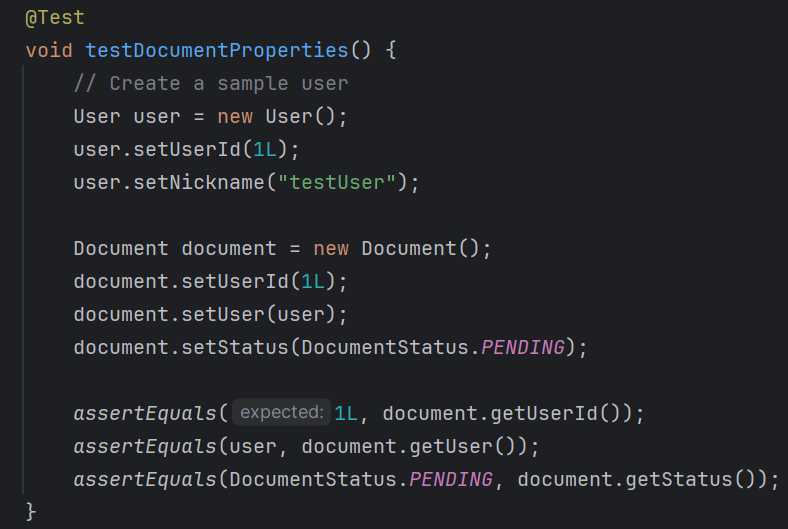
\includegraphics[width=1\linewidth]{slike/DokumentTest.png}


            \subsection{Ispitni slučaj 2.: Test provjere funkcionalnosti ImageChangeRequestStatus}

                                    \textbf{Ulaz:}
                                    \textit{1. Nema posebnog ulaza jer testira vrijednosti unutar samog enuma}

                                    \textbf{Očekivani rezultati:}
                                    \textit{1. Očekujemo da će vrijednosti enuma biti ispravno postavljene.}
                                    \textit{2. Očekujemo da će konverzija enuma u String biti ispravna.}

                                    \textbf{Rezultat:}
                                    \textit{1. Izvršavanje testa provjerava da li su vrijednosti enuma ImageChangeRequestStatus ispravno postavljene}
                                    ~textit{2. Izvršavanje testa provjerava da li je konverzija enuma ImageChangeRequestStatus u String ispravna}

            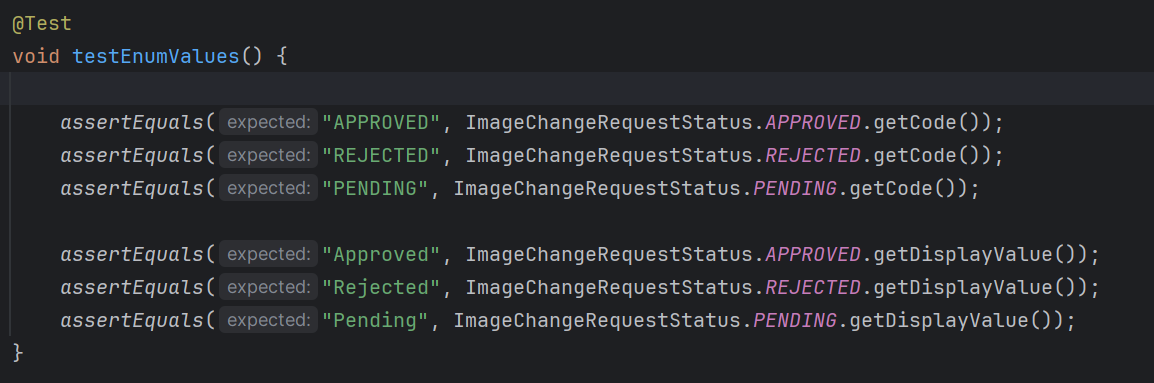
\includegraphics[width=1\linewidth]{slike/ImageChangeTest.png}
            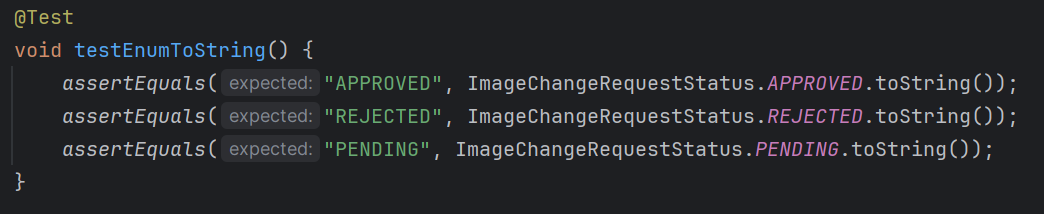
\includegraphics[width=1\linewidth]{slike/ImageChangeTest1.png}

			\subsection{Ispitni slučaj 3.: Provjera Vraćanja Vremena u Razredu Listing}

                                                \textbf{Ulaz:}
                                                \textit{1. Stvaranje instance razreda Listing}
                                                \textit{2. Postavljanje vremena povratka (returnByTime) na trenutno vrijeme}

                                                \textbf{Očekivani rezultati:}
                                                \textit{1. Očekujemo da će vrijeme povratka biti jednako trenutnom vremenu u obliku Timestamp objekta}
                                                \textit{2. Očekujemo da će vrijednost vremena povratka biti null, budući da nije postavljena}


                                                \textbf{Rezultat:}
                                                \textit{1. Izvršavanje testa provjerava postavljanje i dohvaćanje vremena povratka, uspoređujući ga s očekivanim rezultatom}

                                                \textit{2. Izvršavanje testa provjerava da li je vrijednost vremena povratka null, što ukazuje na ispravno ponašanje u slučaju ne postavljanja vremena povratka}

            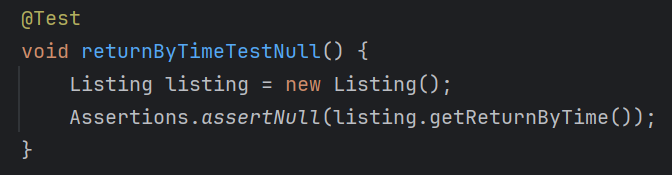
\includegraphics[width=1\linewidth]{slike/ListingTest.png}
            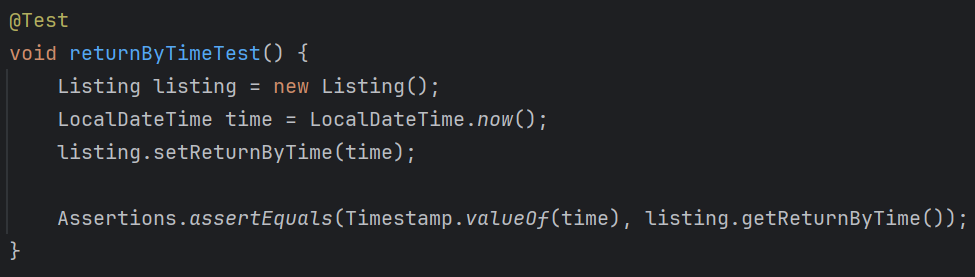
\includegraphics[width=1\linewidth]{slike/ListingTest1.png}

			\subsection{Ispitni slučaj 4.: Test provjere svojstava skutera}

                                                            \textbf{Ulaz:}
                                                            \textit{1. Stvaranje primjerka korisnika (User) i postavljanje njegovih svojstava (ID i nadimak)}

                                                            \textit{2. Stvaranje primjerka skutera (Scooter) i postavljanje njegovih svojstava (ID, proizvođač, model, kapacitet baterije, maksimalna brzina, putanja do slike, maksimalni doseg, godina proizvodnje, dodatne informacije, korisnik, dostupnost)}

                                                            \textbf{Očekivani rezultati:}
                                                            \textit{1. Očekujemo da će svojstva skutera biti ispravno postavljena prema unesenim vrijednostima.}

                                                            \textbf{Rezultat:}
                                                            \textit{1. Izvršavanje testa provjerava ispravnost postavljanja svojstava skutera i uspoređuje ih s očekivanim rezultatima.}

            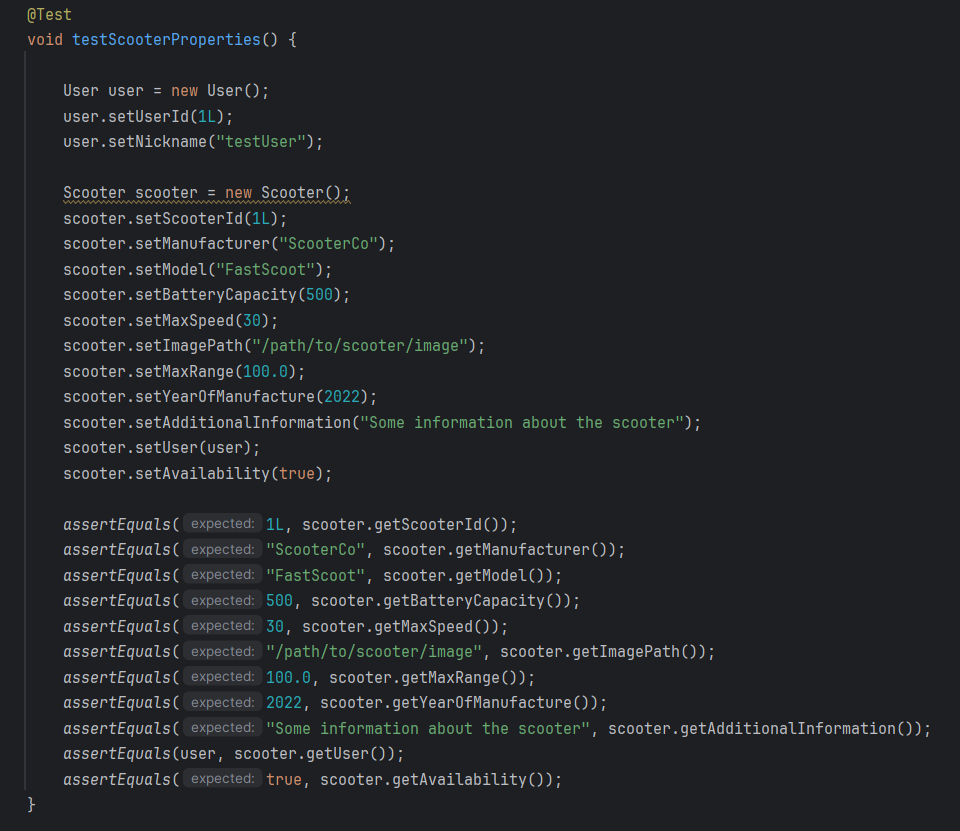
\includegraphics[width=1\linewidth]{slike/ScooterTest.png}

			\subsection{Ispitni slučaj 5.: Test provjere vremena plaćanja u razredu transakcije}

                                                                        \textbf{Ulaz:}
                                                                        \textit{1. Stvaranje instance razreda Transaction}
                                                                        \textit{2. Postavljanje vremena plaćanja (paymentTime) na trenutno vrijeme}

                                                                        \textbf{Očekivani rezultati:}
                                                                        \textit{1. Očekujemo da će vrijeme plaćanja biti jednako trenutnom vremenu u obliku Timestamp objekta}
                                                                        \textit{2. Očekujemo da će vrijednost vremena plaćanja biti null, budući da nije postavljena}


                                                                        \textbf{Rezultat:}
                                                                        \textit{1. Izvršavanje testa provjerava postavljanje i dohvaćanje vremena plaćanja, uspoređujući ga s očekivanim rezultatom}
                                                                        \textit{2. Izvršavanje testa provjerava da li je vrijednost vremena plaćanja null, što ukazuje na ispravno ponašanje u slučaju ne postavljanja vremena plaćanja.}


            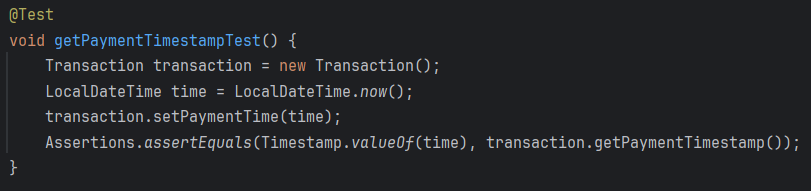
\includegraphics[width=1\linewidth]{slike/TransactionTest.png}
            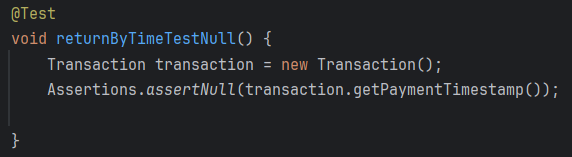
\includegraphics[width=1\linewidth]{slike/TransactionTest1.png}


            \subsection{Ispitni slučaj 6.: Test provjere svojstva korisnika}

                                                                                    \textbf{Ulaz:}
                                                                                    \textit{1. Stvaranje primjerka korisnika (User) i postavljanje njegovih svojstava (ID, nadimak, ime, prezime, broj kartice, e-mail, broj telefona, lozinka, uloga, status)}

                                                                                    \textbf{Očekivani rezultati:}
                                                                                    \textit{1. Očekujemo da će svojstva korisnika biti ispravno postavljena prema unesenim vrijednostima}

                                                                                    \textbf{Rezultat:}
                                                                                    \textit{1. Izvršavanje testa provjerava ispravnost postavljanja svojstava korisnika i uspoređuje ih s očekivanim rezultatima}


            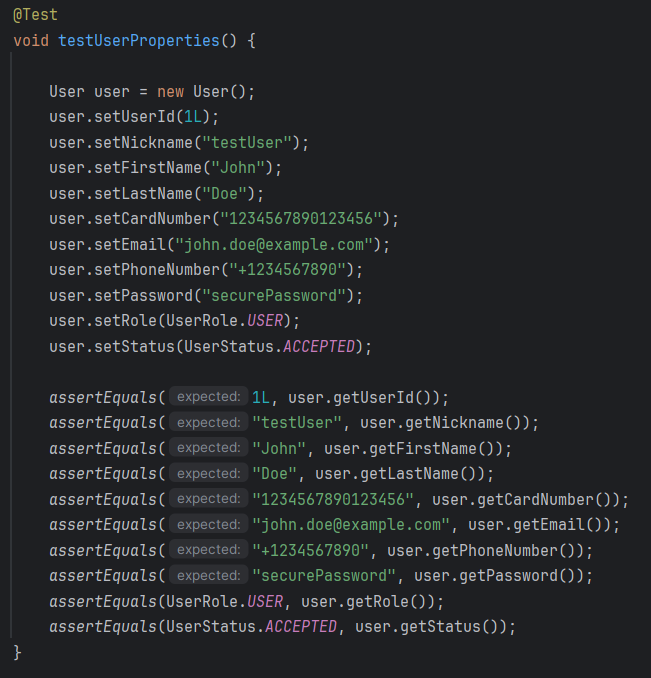
\includegraphics[width=1\linewidth]{slike/UserTest.png}


            \subsection{Ispitni slučaj 7.: Test provjere funkcionalnosti prijave korisnika}

                                                                                                \textbf{Ulaz:}
                                                                                                \textit{1. Koristi se Mock objekt UserRepository}
                                                                                                \textit{2. Koristi se UserService objekt, gdje je userService injektiran u UserService pomoću @InjectMocks}
                                                                                                \textit{3. Postavlja se Mock korisnik (mockUser) s podacima za prijavu}


                                                                                                \textbf{Očekivani rezultati:}
                                                                                                \textit{1. Očekuje se da će korisničko ime i lozinka odgovarati podacima Mock korisnika}
                                                                                                \textit{2. Očekuje se da će userService uspješno vratiti Mock korisnika}


                                                                                                \textbf{Rezultat:}
                                                                                                \textit{1. Izvršava se prijava korisnika pomoću userService.login("test@example.com", "password")}
                                                                                                \textit{2. Provjerava se je li rezultat jednak Mock korisniku (mockUser)}

                        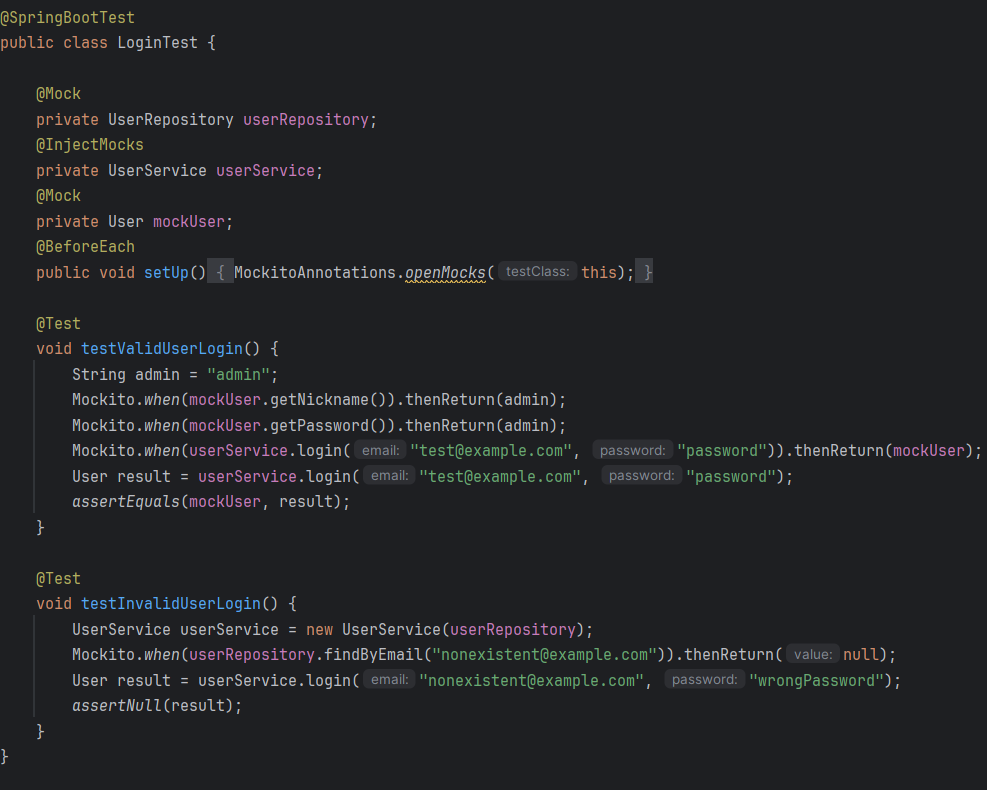
\includegraphics[width=1\linewidth]{slike/LoginTest.png}



			\subsection{Ispitivanje sustava}



			\subsection{Ispitni slučaj 1: provjera ispravnosti registracije}

                                                            \textbf{Cilj:}
                                                            \textit{Automatsko testiranje procesa registracije novog korisnika koji ne unese broj mobitela na web stranici pomoću Selenium WebDriver s Chrome preglednikom.}

                                                            \textbf{Koraci testiranja:}
                                                            \textit{1. Navigacija na stranicu za registraciju}
                                                            \textit{2. Ispunjavanje svih polja registracijskog obrazca osim polja za broj mobitela}
                                                            \textit{3. Potvrda Registracije}
                                                            \textit{4. Provjera je li se korisnik registrirao}


                                                            \textbf{Očekivani rezultati:}
                                                            \textit{1. Korisnik se nije uspio registrirati}
                                                            \textit{2. Ispisana odgovarajuća poruka}


                        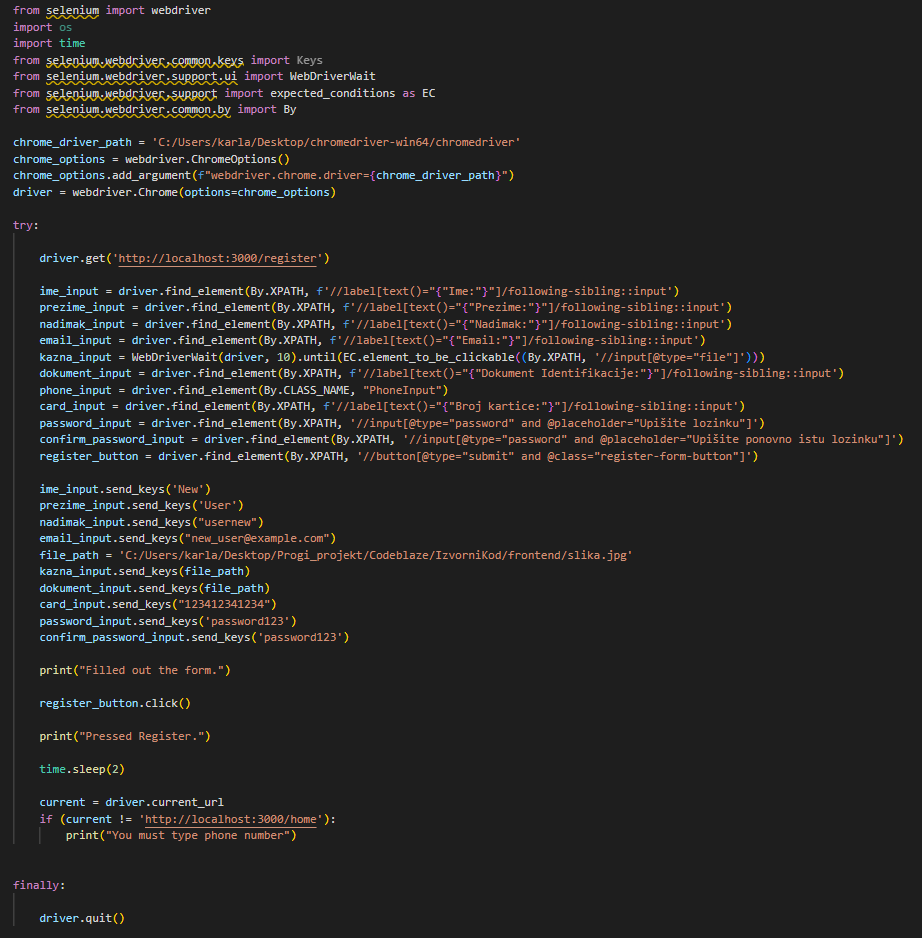
\includegraphics[width=1\linewidth]{slike/RegisterSelenium.png}
                        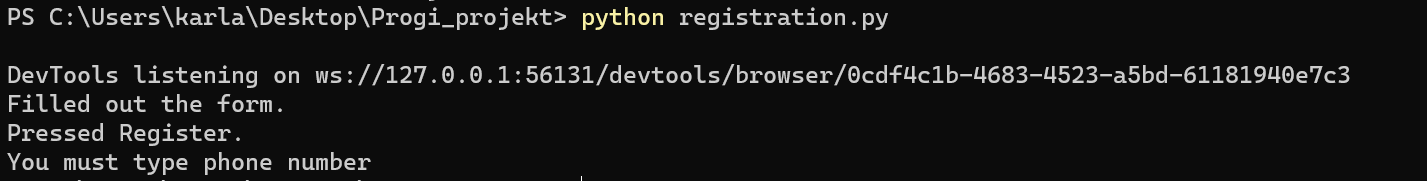
\includegraphics[width=1\linewidth]{slike/RegisterSeleniumOutput.png}


            \subsection{Ispitni slučaj 2: provjera ispravnosti prijave}

                        \textit{Ovaj Selenium test simulira korisničku prijavu na web stranici, unoseći korisničko ime i lozinku te provjerava očekivani rezultat, tj. naslov stranice nakon prijave.}

                                                                        \textbf{Cilj:}
                                                                        \textit{Automatsko testiranje procesa prijavljivanja na web stranicu pomoću Selenium WebDriver s Chrome preglednikom.}

                                                                        \textbf{Koraci testiranja:}
                                                                        \textit{1. Navigacija na stranicu za prijavu}
                                                                        \textit{2. Unos podataka za prijavu}
                                                                        \textit{3. Provjera stranice nakon prijave}


                                                                        \textbf{Očekivani rezultati:}
                                                                        \textit{1. Poruka "Assertion successful: 'Codeblaze' is in the title." ispisuje se kao potvrda uspješne prijave.}

                                    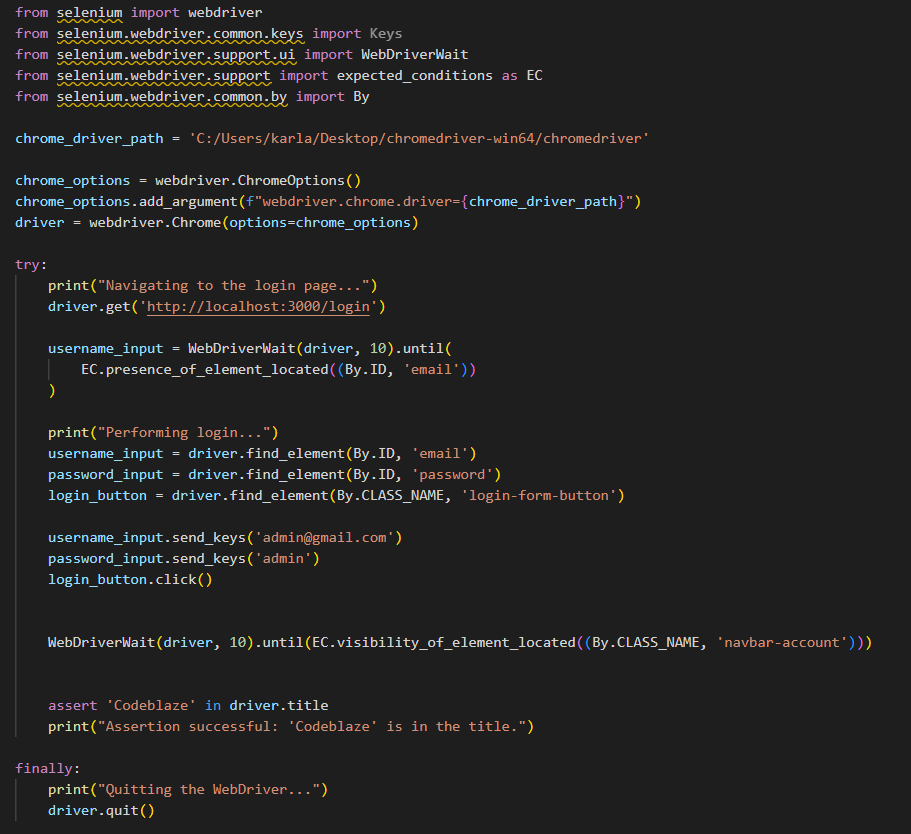
\includegraphics[width=1\linewidth]{slike/LoginSelenium.png}
                                    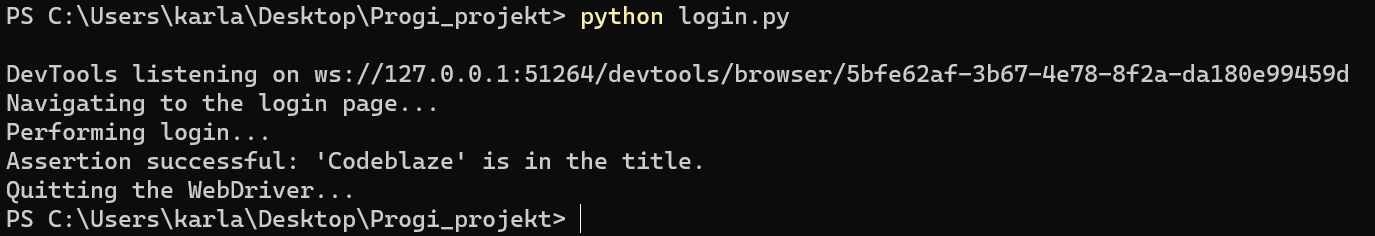
\includegraphics[width=1\linewidth]{slike/LoginSeleniumOutput.png}




			
			\eject 
		
		
		\section{Dijagram razmještaja}
			
			Dijagram rasporeda ilustrira kako su fizički i softverski resursi distribuirani unutar operativnog okvira sustava. Na serveru se smještaju dva ključna servisa: servis za web i servis za upravljanje bazom podataka. Kroz web preglednike, korisnici stječu pristup funkcionalnostima web aplikacije. Ovaj sustav funkcioniše po modelu klijent-server arhitekture gdje je komunikacijski protokol između korisničkih uređaja i servera omogućen putem HTTP veze.

		\begin{figure} [H]
			\centering
			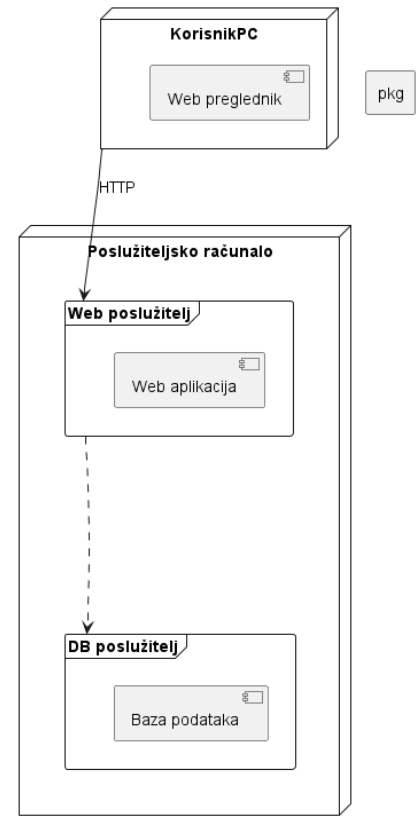
\includegraphics[width=0.7\linewidth]{dijagrami/dijagramRazmjestanja.png}
			\caption{Prikaz dijagrama razmještanja}
			\label{fig:Prikaz dijagrama razmještanja}
		\end{figure}

			\eject 
		
		\section{Upute za puštanje u pogon}

        Nakon što smo temeljito razvili našu aplikaciju, fokusirali smo se na njeno postavljanje u produkcijsko okruženje koristeći Render, cloud-based platformu-as-a-service (PaaS). Postupak smo započeli osiguravanjem da su sve komponente aplikacije pravilno integrirane na GitHubu, čime smo omogućili stvaranje Docker kontejnera ključnih za funkcionalnost naše aplikacije u radnom okruženju. Naš izvorni kod bio je dostupan na GitHub repozitoriju, gdje smo pratili i upravljali verzijama našeg koda.  Izvorni kod naše aplikacije dostupan je na https://github.com/Kvesa- Fer/Codeblaze.

        Prilikom pripreme za deploy, bilo je potrebno dodati environment varijable u run konfiguraciju našeg IDE-a kako bismo osigurali glatko funkcioniranje lokalnog razvojnog okruženja. Posebnu pozornost posvetili smo Dockerfile-u, osiguravajući da su putanje unutar COPY naredbi pravilno postavljene. U našem 'docker' direktoriju nalazile su se dvije verzije Dockerfile-a, za Maven i Gradle, što nam je pružalo fleksibilnost u izboru alata za automatizaciju izgradnje.

        U application.properties datoteci, preporučili smo postavljanje server.servlet.context-path na '/api', što je osiguralo da svi backend zahtjevi budu jasno označeni i usmjereni. Također, opcionalno smo dodali željene environment varijable u formatu some.property=${ENV_VAR_NAME:default value} kako bismo dodatno prilagodili naše okruženje.

        Za lokalni razvoj, integrirali smo Liquibase i H2 bazu, što nam je omogućilo efikasno upravljanje promjenama u strukturi baze podataka i olakšalo razvoj i testiranje aplikacije. Dodavanje odgovarajućih dependency-a u 'pom.xml' i kreiranje 'application-dev.properties' za lokalni dev profil omogućilo nam je brzo prebacivanje između različitih konfiguracija i okruženja.

        Prije deployanja aplikacije, pažljivo smo kreirali bazu podataka na Renderu, postavljajući ime baze i, po potrebi, korisničko ime, dok je lozinka bila automatski generirana. Također, konfiguracija backenda i frontenda na Renderu uključivala je povezivanje s našim GitHub računom, odabir projekta, postavljanje environment varijabli i preciznu konfiguraciju Dockerfile-a.

        Za deploy frontenda, bilo je potrebno dodati neophodne dependency-e u 'package.json', konfigurirati proxy server i postaviti build i start skripte. Nakon tih koraka, aplikacija je bila spremna za pokretanje i bila je dostupna na URL-u koji se generirao nakon deploya na Render platformi.

        Konačna aplikacija dostupna je na poveznici: https://codeblazefe.onrender.com/home.

		\eject